\documentclass[12pt,oneside]{article}
\usepackage[T1]{fontenc}
\usepackage{geometry}
\usepackage{epsfig}
\geometry{verbose,a4paper,tmargin=25mm,bmargin=25mm,lmargin=32mm,rmargin=32mm}
\usepackage{setspace}
\usepackage{amsmath}
\usepackage{enumerate}
\usepackage{amssymb}
\usepackage{graphicx}
\usepackage{float}
\usepackage{xcolor}
\usepackage{tabularray}
\usepackage{array}
\usepackage{ragged2e}
\usepackage{pdflscape}
\usepackage{longtable}
\usepackage{tabularx}


\setcounter{secnumdepth}{5}
\setcounter{tocdepth}{5}
\usepackage{txfonts}
% \usefont{T1}{tnr}{m}{sl}
\makeatletter
\makeatother
\renewcommand{\contentsname}{TABLE OF CONTENTS}
% \renewcommand\listtablename{LIST OF TABLES}
% \renewcommand\listfigurename{LIST OF FIGURES}
% \renewcommand\bibname{REFERENCES}
% \usepackage[round, sort]{natbib}
\usepackage[nottoc]{tocbibind}
% \renewcommand{\chaptername}{CHAPTER}
%\renewcommand{\section}{\MakeUppercase}
\usepackage[authoryear,round]{natbib}
% \usepackage[options]{natbib}
\newtheorem{definition}{Definition}
\begin{document}
%%%%%%%%%%%%%%%%%%%%%%%%%%%%%%%%%%%
% Title Page
\title{}
\author{}
\thispagestyle{empty}

\begin{titlepage}
\begin{center}
{\LARGE \bf Project Proposal for Setup of Additional Manufacturing Plant of Patanjali in Surat, Gujarat} \\
\end{center}
\begin{center}
%\vspace{0.2in}
%{\large Dissertation} \\
\vspace{0.6in}
{\LARGE A Project Management Report} \\
\vspace{0.6in}
{\large \it Submitted by\\\vspace{0.1in}}
{\large \bf \vspace{0.2in}Divyanshu\\(2019IMG-018)\\}
\vspace{0.6in}
{\large \it Submitted to\\}
\vspace{0.1in}
{\large \bf Prof. Rajendra Sahu}\\
%{\normalsize (2019IMG-018)}\\
%{\normalsize }\\
\end {center}
\vspace{0.5in}
\begin{figure}[h]
\centerline{
\includegraphics[width=1.2in]{./iiitm}}
\end{figure}
%\vspace{0.1in}
\begin{center}
{\Large \bf ABV INDIAN INSTITUTE OF INFORMATION TECHNOLOGY AND MANAGEMENT\\
GWALIOR-474 015\\}
\vspace{0.2in}
{\Large \bf 2023\\}
\end{center}
\end{titlepage}
%\pagestyle{headings}
%%%%%%%%%%%%%%%%%%%%%%%%%%%%%%%%%%%
\setcounter{page}{1}
\pagenumbering{roman}
%%%%%%%%%%%%%%%%%%%%%%%%%%%%%%%%%%%%%%%%%%%%%%%%%%%%%%%%%%%%%%%%%%%%%%%%%%%%%%
% \newpage
\begin{center}
{\large \bf CANDIDATES DECLARATION}
\end{center}
I hereby certify that the work, which is being presented in the report, entitled {\bf A Comparative Analysis of Deep Learning and Traditional Portfolio Optimization Models in Developed Financial Markets }, in partial fulfilment of the requirement for the award of the
Degree of {\bf Masters of Business Administration} and submitted to the institution is an authentic record of my own work carried out
during the period \emph{June 2023} to \emph{October 2023} under the supervision of {\bf Dr. Vishal Vyas}.
I have also cited the references about the text(s)/figure(s)/table(s) from where they have been taken.\\
\vspace{0.6in} \\
Date: \hspace{3.4in} Signatures of the Candidates \\
%\begin{flushright}
%Signatures of the Candidates
%\end{flushright}
\vspace{0.2in} \\
This is to certify that the above statement made by the candidates is correct to the best of my knowledge. \\
\vspace{0.5in} \\
Date: \hspace{2.65in} Signatures of the Research Supervisor \\
%\begin{flushright}
%Signatures of the Research Supervisors
%\end{flushright}


% 
\newpage
\begin{center}
{\large \bf ACKNOWLEDGEMENTS}
\end{center}
%\textcolor{white}{"\indent}
I am deeply grateful to \textbf{Dr. Vishal Vyas} for his unwavering support and trust in my ability to work independently and explore innovative ideas. I would like to take this opportunity to express my heartfelt appreciation for his invaluable guidance, personal concern for my project, and active support throughout this endeavor. Dr. Vyas's mentoring sessions played a pivotal role in boosting my confidence, instilling a sense of self-assurance, and inspiring me to excel. His direction, recommendations, insightful judgments, constructive criticism, and commitment to excellence have all been instrumental in nurturing and advancing the current work.

I am immensely thankful to my mentor for his graciousness, patience, and willingness to listen to my ideas, always offering praise and constructive refinement. His open-minded approach and trust in my capabilities allowed me the freedom to explore and develop my project to its fullest potential. It is through his constant attention and supportive attitude that this project has reached its current level of accomplishment.

Lastly, I extend my gratitude to our esteemed institution and my colleagues, whose ongoing encouragement rejuvenated my enthusiasm, focused my efforts, and provided essential assistance in completing this undertaking. Your collective support has been instrumental in my journey, and I am sincerely appreciative of your contributions to my success.
\section*{Executive Summary}
This report provides an in-depth analysis of IBM's technology management practices, including its historical background, current state of technology infrastructure and capabilities, and best practices in technology management. The report also highlights the implications of IBM's findings and provides recommendations for the company to maintain its leadership position in key technology areas.

IBM is a technology company that has been at the forefront of innovation for over a century. The company's technology initiatives have evolved over time, from tabulating machines to mainframes, personal computers, and cloud computing. IBM's current technology infrastructure and capabilities include hybrid cloud, artificial intelligence (AI), blockchain, quantum computing, and cybersecurity.

IBM's technology management practices are guided by best practices that include a focus on innovation, collaboration, and customer-centricity. The company invests heavily in research and development to maintain its leadership position in key technology areas. IBM also has a strong brand reputation and develops targeted marketing and sales strategies for key customer segments.

The implications of IBM's findings are significant. The company needs to continue investing in research and development to maintain its leadership in key technology areas. IBM should also expand its global reach to tap into new markets and customer segments. Strengthening brand reputation and developing targeted marketing and sales strategies for key customer segments are also essential.

To maintain its leadership position in key technology areas, IBM should invest in hybrid cloud and AI, two of the fastest-growing IT segments. Hybrid cloud is a critical area for IBM, as it enables customers to seamlessly integrate their on-premises and cloud environments. AI is another rapidly growing IT segment that IBM should continue to invest in to maintain its leadership position in this market.

IBM should also focus on developing its blockchain and quantum computing capabilities. Blockchain is a distributed ledger technology that has the potential to transform industries such as finance, healthcare, and supply chain management. Quantum computing is a new computing paradigm that has the potential to solve complex problems that are beyond the capabilities of classical computers.

Finally, IBM should continue to invest in cybersecurity to protect its customers' data and systems. Cybersecurity threats are increasing in frequency and sophistication, and IBM needs to stay ahead of the curve to protect its customers.

In conclusion, IBM's technology management practices are guided by best practices that include a focus on innovation, collaboration, and customer-centricity. The company's current technology infrastructure and capabilities include hybrid cloud, AI, blockchain, quantum computing, and cybersecurity. To maintain its leadership position in key technology areas, IBM should invest in hybrid cloud and AI, focus on developing its blockchain and quantum computing capabilities,

\newpage

%%%%%%%%%%%%%%%%%%%%%%%%%%%%%%%%%%%%%%%%%%%%%%%%%%%%%%%%%%%%%%%%%%%%%%%%%%%%%
\tableofcontents
\setcounter{page}{1}
\pagenumbering{arabic}
% \addcontentsline{toc}{chapter}{LIST OF TABLES}
% \listoftables
% \addcontentsline{toc}{chapter}{LIST OF FIGURES}
% \listoffigures
%%%%%%%%%%%%%%%%%%%%%%%%%%%%%%%%%%%%%%%%%%%%%%%%%%%%%%%%%%%%%%%%%%%%%%%%%%%%%%
\section{Introduction}
\label{introchap}


\subsection{About SMEs}


\subsection{About Thejo Engineering Ltd}

\subsection{Recent Growth Trends of Thejo Engineering Ltd. }
\section{Project Scope}
\subsection{GeM Functionalities}

\begin{enumerate}
    \item \textbf{Catalog Management:} GeM maintains a comprehensive catalog of goods and services, categorized and standardized to facilitate search and comparison. Buyers can easily browse, filter, and compare products based on specifications, pricing, and supplier ratings.
    
    \item \textbf{Supplier Registration and Onboarding:} GeM provides a streamlined supplier registration and onboarding process, enabling businesses to establish their presence on the platform and showcase their offerings. Suppliers must meet specific eligibility criteria and undergo verification procedures to ensure quality and compliance.
    
    \item \textbf{Demand Aggregation and Procurement Planning:} GeM facilitates demand aggregation by enabling buyers to consolidate their requirements and negotiate better prices with suppliers. This bulk buying approach leads to cost savings and efficient resource utilization.
    
    \item \textbf{E-bidding and Reverse Auction:} GeM supports electronic bidding and reverse auction mechanisms, allowing buyers to invite bids from multiple suppliers and secure the best possible price. These competitive bidding processes promote transparency and efficiency.
    
    \item \textbf{Order Management and Contract Award:} GeM streamlines order management by providing a secure channel for buyers to place orders, track deliveries, and manage contract terms. Contract awards are based on predefined criteria and transparent bidding processes.
    
    \item \textbf{E-payment and Payment Management:} GeM integrates electronic payment gateways, enabling secure and convenient payments for goods and services procured through the platform. This integration reduces the need for cash transactions and enhances financial traceability.
    
    \item \textbf{Performance Monitoring and Feedback Mechanism:} GeM incorporates a performance monitoring system that tracks supplier performance based on order fulfillment, delivery timelines, and quality of products. Buyers can provide feedback and ratings, influencing supplier rankings and future procurement decisions.
    
    \item \textbf{Data Analytics and Reporting:} GeM generates comprehensive data and reports on procurement activities, providing insights into spending patterns, supplier performance, and market trends. This information can inform strategic procurement decisions and improve resource allocation.
    
    \item \textbf{User Management and Access Control:} GeM implements a robust user management system with granular access control permissions, ensuring that only authorized individuals can access sensitive procurement information. This system protects data integrity and prevents unauthorized access.
    
    \item \textbf{Grievance Redressal Mechanism:} GeM establishes a grievance redressal mechanism to address complaints and concerns raised by buyers, suppliers, or other stakeholders. This mechanism ensures transparency and accountability in the procurement process.
\end{enumerate}

\subsection{GeM Initiatives}

\begin{enumerate}
    \item \textbf{MSME Empowerment:} GeM prioritizes the participation of Micro, Small, and Medium Enterprises (MSMEs) by providing a level playing field and facilitating their access to government procurement opportunities. This empowerment supports MSME growth and economic development.
    
    \item \textbf{Local Supplier Promotion:} GeM encourages the procurement of goods and services from local suppliers, fostering regional development and economic inclusion. This focus on local suppliers strengthens local economies and reduces reliance on external supply chains.
    
    \item \textbf{Sustainable Procurement Practices:} GeM promotes environmentally friendly and sustainable procurement practices by encouraging the purchase of eco-friendly products and services. This focus on sustainability contributes to environmental protection and resource conservation.
    
    \item \textbf{Technology Adoption and Innovation:} GeM embraces technological advancements to enhance procurement efficiency and transparency. It explores emerging technologies such as artificial intelligence and machine learning to optimize processes and improve decision-making.
    
    \item \textbf{Stakeholder Engagement and Outreach:} GeM engages with various stakeholders, including government buyers, suppliers, industry associations, and civil society organizations, to gather feedback, address concerns, and promote best practices in public procurement.
\end{enumerate}

The scope of the GeM project is continuously evolving, adapting to changing market dynamics, technological advancements, and government policies. It strives to remain a transformative force in public procurement, driving efficiency, transparency, and inclusivity in the Indian government's procurement landscape.


\subsection{Inclusion and Exclusion Criteria in GeM}

The Government e-Marketplace (GeM) has established inclusion and exclusion criteria to ensure that only eligible suppliers and buyers can participate in the procurement process. These criteria are designed to maintain the integrity of the platform and promote fair competition among suppliers.

\subsubsection{Inclusion Criteria}

To be eligible to register as a seller on GeM, a supplier must meet the following general inclusion criteria:

\begin{enumerate}
    \item \textbf{Legal Entity:} The supplier must be a legally registered entity in India, such as a sole proprietorship, partnership, company, or LLP.
    
    \item \textbf{PAN and TAN:} The supplier must possess a valid Permanent Account Number (PAN) and Tax Deduction and Account Number (TAN) issued by the Income Tax Department of India.
    
    \item \textbf{GST Registration:} The supplier must be registered for Goods and Services Tax (GST) in India, unless exempted under specific provisions.
    
    \item \textbf{Bank Account:} The supplier must maintain a valid bank account in India linked to their PAN.
    
    \item \textbf{Category-Specific Requirements:} In addition to these general criteria, some categories of goods and services may have additional eligibility requirements, such as specific licenses or certifications.
\end{enumerate}

\subsubsection{Exclusion Criteria}

Certain suppliers are not eligible to register on GeM or participate in procurement activities. These exclusion criteria are designed to prevent conflicts of interest, maintain ethical standards, and protect the interests of the government and other stakeholders.

\begin{enumerate}
    \item \textbf{Government Entities:} Government departments, organizations, or PSUs are not allowed to register as sellers on GeM.
    
    \item \textbf{Insolvent or Bankrupt Entities:} Suppliers declared insolvent or bankrupt under applicable laws are not eligible to participate in GeM.
    
    \item \textbf{Blacklisted Suppliers:} Suppliers blacklisted or debarred by government agencies or courts for procurement-related irregularities are not allowed on GeM.
    
    \item \textbf{Tax Defaulters:} Suppliers with outstanding tax liabilities or a history of tax evasion are not eligible to participate in GeM.
    
    \item \textbf{Conflict of Interest:} Suppliers with a direct or indirect conflict of interest with government officials or procurement processes are not allowed on GeM.
    
    \item \textbf{Category-Specific Exclusions:} Some categories of goods and services may have additional exclusion criteria, such as restrictions on the sale of certain products or services.
\end{enumerate}

\subsubsection{Verification and Monitoring}

GeM employs a combination of automated and manual verification processes to ensure compliance with inclusion and exclusion criteria. Suppliers must submit relevant documents and undergo verification checks before being approved for registration.

GeM also continuously monitors supplier activities and performance to detect any violations of inclusion and exclusion criteria. Upon identification of a violation, GeM may take appropriate action, including suspension or termination of the supplier's account.

\subsubsection{Importance of Inclusion and Exclusion Criteria}

Inclusion and exclusion criteria play a crucial role in maintaining the integrity and effectiveness of the GeM platform. By ensuring that only eligible and responsible suppliers participate in the procurement process, GeM safeguards the interests of government buyers and promotes fair competition.

These criteria also contribute to ethical and transparent procurement practices, reducing the risk of corruption and promoting good governance in the Indian government's procurement system.


\subsection{Key Expected Outcomes of GeM}

\begin{enumerate}
    \item \textbf{Enhanced Efficiency and Cost Savings:} GeM aims to streamline procurement processes, reduce administrative burdens, and promote competition among suppliers, leading to lower procurement costs for the government.
    
    \item \textbf{Increased Transparency and Accountability:} GeM strives to make the procurement process more transparent by providing open access to bidding information, contract awards, and supplier performance data. This transparency promotes accountability and reduces opportunities for corruption.
    
    \item \textbf{Expanded Market Access and Competition:} GeM aims to create a level playing field for all suppliers, regardless of their size or connections, providing wider market access and encouraging competition. This open and competitive environment is expected to drive innovation and lower prices.
    
    \item \textbf{Empowerment of Small and Medium Enterprises (SMEs):} GeM seeks to provide SMEs with a direct and cost-effective channel to participate in government procurement, boosting their growth and contribution to the Indian economy.
    
    \item \textbf{Improved Demand Aggregation and Price Discovery:} GeM aims to improve demand aggregation and price discovery by providing a centralized platform for buyers to consolidate their requirements and negotiate better prices.
    
    \item \textbf{Adoption of E-payment Methods:} GeM encourages the adoption of e-payment methods for procurement transactions, reducing the use of cash and improving transaction security.
    
    \item \textbf{Promotion of Local Suppliers and Regional Development:} GeM seeks to encourage the procurement of goods and services from local suppliers, fostering regional development and economic inclusion.
    
    \item \textbf{Reduction in Administrative Burdens and Transaction Costs:} GeM aims to reduce administrative burdens and transaction costs for both buyers and sellers by automating many of the procurement tasks and providing a centralized platform for communication and collaboration.
    
    \item \textbf{Data-driven Decision Making:} GeM seeks to improve data analytics and performance monitoring to identify trends, optimize procurement strategies, and make informed decisions.
    
    \item \textbf{Enhanced User Experience and Accessibility:} GeM aims to provide a user-friendly and accessible platform for all stakeholders involved in the procurement process.
    
    \item \textbf{Innovation and Technology Adoption:} GeM seeks to promote innovation and technology adoption in the procurement process, leading to more efficient and effective practices.
\end{enumerate}

\subsection{Expected Deliverables of GeM}

The implementation of GeM is expected to deliver a range of tangible outcomes, including:

\begin{enumerate}
    \item \textbf{Reduction in Procurement Costs:} GeM is expected to lead to significant cost savings for the government by streamlining processes, reducing administrative burdens, and promoting competition.
    
    \item \textbf{Increase in Transparency:} GeM's open and transparent platform is expected to increase transparency in public procurement, reducing opportunities for corruption and improving accountability.
    
    \item \textbf{Wider Market Access for Suppliers:} GeM is expected to provide wider market access for suppliers, particularly SMEs, leading to increased competition and innovation.
    
    \item \textbf{Empowerment of SMEs:} GeM is expected to empower SMEs by providing them with a direct and cost-effective channel to participate in government procurement.
    
    \item \textbf{Improved Price Discovery:} GeM's centralized platform is expected to improve price discovery by providing buyers with access to a wider range of suppliers and real-time price comparisons.
    
    \item \textbf{Adoption of E-payment Methods:} GeM is expected to encourage the adoption of e-payment methods for procurement transactions, reducing the use of cash and improving transaction security.
    
    \item \textbf{Promotion of Local Suppliers:} GeM is expected to promote the procurement of goods and services from local suppliers, fostering regional development and economic inclusion.
    
    \item \textbf{Reduction in Transaction Costs:} GeM is expected to reduce transaction costs for both buyers and sellers by automating many of the procurement tasks and providing a centralized platform for communication and collaboration.
    
    \item \textbf{Improved Decision Making:} GeM's data analytics and performance monitoring tools are expected to improve decision making by providing insights into procurement trends and supplier performance.
    
    \item \textbf{Enhanced User Experience:} GeM's user-friendly and accessible platform is expected to improve the user experience for all stakeholders involved in the procurement process.
    
    \item \textbf{Adoption of Innovative Technologies:} GeM is expected to promote the adoption of innovative technologies in the procurement process, leading to more efficient and effective practices.
\end{enumerate}

\subsection{Measuring the Impact of GeM}

To evaluate the impact of GeM, the government has established a set of performance indicators and targets. These indicators measure key aspects of procurement performance, such as cost savings, transparency, competition, and SME participation. Regular monitoring and evaluation of these indicators will help assess the effectiveness of GeM and identify areas for improvement.

The implementation of GeM is a significant step forward in modernizing public procurement in India. It is expected to bring about a range of positive outcomes, including increased efficiency, transparency, competition, and inclusivity. By delivering on its expected outcomes, GeM aims to transform the public procurement landscape and contribute to the overall development of the Indian economy.

\section{Conceptualization Phase}
The Government e-Marketplace (GeM) project was conceived out of the need to modernize and streamline public procurement in India. The traditional procurement system was fragmented, manual, and lacked transparency, leading to inefficiencies, corruption, and higher costs.



\subsection{Initial Discussions and Brainstorming}

The initial discussions on the GeM project idea began in the early 2010s, within the Directorate General of Supplies and Disposals (DGS\&D), a central government organization responsible for procurement for the Indian government. Recognizing the challenges of the traditional system, DGS\&D officials began exploring the possibility of developing a centralized e-procurement platform.

These initial discussions involved brainstorming sessions with experts from various fields, including technology, procurement, and law. The aim was to gather insights and perspectives on how to design an effective e-procurement platform that could address the shortcomings of the existing system.

\begin{itemize}
    \item \textbf{Scope of the Platform:} Determining the scope of the platform, including the range of goods and services to be covered, the types of buyers and sellers to be involved, and the geographical reach of the platform.
    
    \item \textbf{Technical Requirements:} Defining the technical requirements for the platform, such as the software architecture, security protocols, and user interface design.
    
    \item \textbf{Legal and Regulatory Framework:} Ensuring compliance with existing laws and regulations governing public procurement, data privacy, and electronic transactions.
    
    \item \textbf{Change Management:} Addressing the challenges of change management, including training and onboarding of buyers and sellers, overcoming resistance to new technologies, and adapting to new procurement processes.
\end{itemize}

\subsection{Formulating a Project Plan}

Based on the insights gained from these initial discussions, DGS\&D officials began formulating a project plan for the development and implementation of GeM. This plan included defining project objectives, identifying resource requirements, establishing timelines, and outlining a strategy for stakeholder engagement.

\subsection{Engaging Stakeholders and Seeking Feedback}

Throughout the project planning process, DGS\&D engaged with various stakeholders, including government departments, industry associations, and supplier representatives. Their feedback was sought on various aspects of the project, such as the platform's design, features, and usability.

\subsection{Securing Government Approval}

To secure government approval for the GeM project, DGS\&D prepared a detailed proposal outlining the project's objectives, benefits, and implementation plan. The proposal was presented to the Ministry of Finance and other relevant ministries, who reviewed the proposal and provided feedback.

\subsection{Pilot Testing and Refinement}

Before launching GeM on a full-scale basis, DGS\&D conducted a pilot test in a limited number of government departments and with a select group of suppliers. This pilot testing allowed for identifying and addressing any technical glitches, usability issues, or process bottlenecks.

\subsection{Launch and Initial Rollout}

The GeM project was officially launched in 2016, and the platform was initially rolled out to a limited number of government departments and categories of goods and services. Over time, the platform's scope was expanded to include more categories, buyers, and sellers.

\subsection{Continuous Improvement and Expansion}

Since its launch, GeM has undergone continuous improvement and expansion. New features have been added, user interfaces have been refined, and the platform's reach has been extended to all government departments, organizations, and PSUs across India.

\subsection{GeM as a Transformative Force in Public Procurement}

GeM has played a transformative role in modernizing public procurement in India. It has brought about a shift from the traditional manual and fragmented system to a centralized, transparent, and efficient e-procurement platform. GeM has contributed to significant cost savings, increased competition, and enhanced accountability in public procurement.

\section{Planning Phase}

\subsection{Activities Involved in the GeM Project}

\subsubsection{Project Planning and Definition}

\begin{itemize}
    \item \textbf{Identifying Needs and Objectives:} This initial phase involved understanding the shortcomings of the traditional procurement system and defining the specific goals and objectives of the GeM project.
    
    \item \textbf{Stakeholder Engagement:} DGS\&D engaged with various stakeholders, including government departments, industry associations, and supplier representatives, to gather input and feedback on the project's design and implementation.
    
    \item \textbf{Feasibility Study and Requirements Gathering:} A comprehensive feasibility study was conducted to assess the technical, financial, and operational viability of the project. Detailed requirements were gathered from stakeholders to inform the platform's design and functionality.
\end{itemize}

\subsubsection{Design and Development}

\begin{itemize}
    \item \textbf{Technical Architecture and Infrastructure:} The technical architecture of the GeM platform was designed to ensure scalability, security, and reliability. The project team also planned and implemented the necessary IT infrastructure to support the platform.
    
    \item \textbf{Software Development and Testing:} A team of software developers was assembled to design, develop, and test the GeM platform. The platform underwent rigorous testing to ensure functionality, performance, and security.
    
    \item \textbf{User Interface and User Experience Design:} A user-centric approach was adopted to design the GeM platform's interface, ensuring ease of use and accessibility for buyers, sellers, and other stakeholders.
\end{itemize}

\subsubsection{Implementation and Deployment}

\begin{itemize}
    \item \textbf{Pilot Testing and Refinement:} Before full-scale deployment, GeM underwent pilot testing in a limited number of government departments and with a select group of suppliers. This testing allowed for identifying and addressing any technical glitches, usability issues, or process bottlenecks.
    
    \item \textbf{Training and Onboarding:} Comprehensive training programs were conducted for government buyers and suppliers to familiarize them with the GeM platform's features, functionalities, and procurement processes.
    
    \item \textbf{Rollout and Expansion:} GeM was initially rolled out to a limited number of government departments and categories of goods and services. Over time, the platform's scope was expanded to include more categories, buyers, and sellers.
\end{itemize}

\subsubsection{Ongoing Maintenance and Improvement}

\begin{itemize}
    \item \textbf{Performance Monitoring and Analytics:} GeM implemented a robust performance monitoring system to track key metrics, such as transaction volume, user engagement, and supplier performance. This data was used to identify areas for improvement and optimize the platform's performance.
    
    \item \textbf{User Feedback and Issue Resolution:} A dedicated feedback mechanism was established to collect user feedback and address any issues or concerns raised by buyers, sellers, or other stakeholders.
    
    \item \textbf{Continuous Enhancements and Updates:} GeM underwent regular updates and enhancements to incorporate new features, improve user experience, and address evolving procurement needs.
\end{itemize}

\subsection{Timeframe for the Execution of GeM}

\subsubsection{Phase 1: Project Planning and Definition}

\begin{itemize}
    \item Needs assessment and objective setting
    \item Stakeholder engagement and requirements gathering
    \item Feasibility study and project planning
\end{itemize}

\subsubsection{Phase 2: Design and Development}

\begin{itemize}
    \item Technical architecture and infrastructure planning
    \item Software development and testing
    \item User interface and user experience design
\end{itemize}

\subsubsection{Phase 3: Implementation and Deployment}

\begin{itemize}
    \item Pilot testing and refinement
    \item Training and onboarding of buyers and sellers
    \item Full-scale rollout and expansion
\end{itemize}

\subsubsection{Phase 4: Ongoing Maintenance and Improvement}

\begin{itemize}
    \item Performance monitoring and analytics
    \item User feedback and issue resolution
    \item Continuous enhancements and updates
\end{itemize}

\subsection{Sequencing of Activities for GeM Implementation}

\begin{enumerate}
    \item Establish Project Management Structure and Team: A dedicated project management team was formed to oversee the project's execution, ensuring coordination and accountability across various phases.
    
    \item Define Project Scope and Requirements: The project's scope was clearly defined, outlining the specific functionalities, features, and user groups that GeM would cater to. Detailed requirements were gathered from stakeholders to guide the platform's design and development.
    
    \item Conduct Market Research and Benchmarking: Market research was conducted to assess existing e-procurement solutions and identify best practices. Benchmarking against leading e-procurement platforms helped in setting high standards for GeM's design and performance.
    
    \item Develop Technical Architecture and Infrastructure: The technical architecture of the GeM platform was designed to meet scalability, security, and reliability requirements. The necessary IT infrastructure was planned and implemented to support the platform's operation.
    
    \item Design and Develop Software Components: The software development team followed an iterative approach, designing, developing, and testing each component of the GeM platform. Rigorous testing ensured that the platform met all functional, performance, and security requirements.
    
    \item Prepare Training Materials and Conduct Onboarding: Comprehensive training materials were prepared to familiarize government buyers and sellers with the GeM platform's features, functionalities, and procurement processes. Onboarding sessions were conducted to guide users through the platform and address any initial questions or concerns.
    
    \item Conduct Pilot Testing and Refinement: Before full-scale deployment, GeM underwent pilot testing in a limited number of government departments and with a select group of suppliers. This testing allowed for identifying and addressing any technical glitches, usability issues, or process bottlenecks.
    
    \item Initiate Full-Scale Rollout and Expansion: Based on the learnings from pilot testing, GeM was rolled out to a larger number of government departments and categories of goods and services. The platform's scope was gradually expanded to include more buyers, sellers, and product categories.
    
    \item Establish Performance Monitoring and Analytics: A robust performance monitoring system was implemented to track key metrics, such as transaction volume, user engagement, and supplier performance. This data was used to identify areas for improvement and optimize the platform's performance.
    
    \item Implement User Feedback Mechanism and Issue Resolution: A dedicated feedback mechanism was established to collect user feedback and address any issues or concerns raised by buyers, sellers, or other stakeholders. Prompt response to feedback ensured that the platform continued to meet user needs and expectations.
    
    \item Plan and Implement Ongoing Enhancements: GeM underwent regular updates and enhancements to incorporate new features, improve user experience, and address evolving procurement needs. A roadmap for future enhancements was developed to ensure that the platform remained at the forefront of e-procurement technology.
\end{enumerate}

\subsection{Estimation of Project Scope and Complexity}

The GeM project was a large and complex undertaking, encompassing various aspects of public procurement, from software development and infrastructure setup to user training and ongoing maintenance. The project scope can be summarized as follows:

\begin{itemize}
    \item \textbf{Platform Development:} Development of a comprehensive e-procurement platform with a wide range of functionalities, including buyer and seller registration, product catalog management, bidding and auction mechanisms, order processing, and payment settlement.
    
    \item \textbf{Infrastructure Setup:} Procurement and deployment of hardware and software infrastructure to support the platform, including servers, network equipment, and data security systems.
    
    \item \textbf{User Training and Onboarding:} Training and onboarding of government buyers, suppliers, and other stakeholders on the use of the GeM platform and the new procurement processes.
    
    \item \textbf{Ongoing Maintenance and Support:} Ongoing maintenance of the platform to address technical issues, implement updates, and ensure optimal performance.
\end{itemize}

\subsection{Budgeting for Project Execution}

The GeM project involved significant financial investments to cover the costs of software development, hardware procurement, training, and ongoing maintenance. The estimated budget for the project can be broken down as follows:

\begin{itemize}
    \item \textbf{Software Development:} \rupee300 crore to \rupee400 crore
    
    \item \textbf{Hardware Procurement:} \rupee100 crore to \rupee150 crore
    
    \item \textbf{Training and Onboarding:} \rupee50 crore to \rupee75 crore
    
    \item \textbf{Ongoing Maintenance and Support:} \rupee50 crore to \rupee75 crore per year
\end{itemize}

\subsection{Staffing Requirements for Project Implementation}

The GeM project required a diverse team of experts with specialized skills and experience in various domains, including software development, IT infrastructure, training, and public procurement. The estimated staffing requirements for the project can be categorized as follows:

\begin{itemize}
    \item \textbf{Software Development Team:} 50-75 software developers, including architects, designers, and testers
    
    \item \textbf{IT Infrastructure Team:} 10-15 IT infrastructure specialists, including network engineers, system administrators, and security experts
    
    \item \textbf{Training and Onboarding Team:} 20-30 trainers and support staff
    
    \item \textbf{Public Procurement Experts:} 10-15 procurement specialists to provide guidance and support on procurement processes and best practices
\end{itemize}

\subsection{Project Timeline and Milestones}

The GeM project was executed in phases, with specific milestones and deliverables defined for each phase. The estimated timeframe for the project can be outlined as follows:

\begin{itemize}
    \item \textbf{Phase 1: Project Planning and Design (12-18 months)}
    
    \begin{itemize}
        \item Needs assessment, objective setting, and stakeholder engagement
        \item Feasibility study and technical architecture design
        \item Detailed software requirements and user interface design
    \end{itemize}
    
    \item \textbf{Phase 2: Software Development and Testing (24-36 months)}
    
    \begin{itemize}
        \item Development of platform components and functionalities
        \item Rigorous testing and quality assurance
        \item User acceptance testing and refinement
    \end{itemize}
    
    \item \textbf{Phase 3: Pilot Testing and Implementation (6-12 months)}
    
    \begin{itemize}
        \item Pilot testing in a limited number of government departments and with select suppliers
        \item Identification and resolution of technical glitches and usability issues
        \item Gradual rollout to a wider range of users and product categories
    \end{itemize}
    
    \item \textbf{Phase 4: Ongoing Maintenance and Improvement (Continuous)}
    
    \begin{itemize}
        \item Performance monitoring and analytics
        \item User feedback and issue resolution
        \item Regular updates and enhancements based on evolving procurement needs
    \end{itemize}
\end{itemize}

\section{Critical Success Factors of Construction Company}

\begin{enumerate}
    \item Management Commitments
    \item Financial Perspective
    \item Mutual vision, goals and objectives
    \item Trust
    \item Continuous evaluation/improvement of performance
    \item Good Communication 
    \item Conflict resolution processes 
    \item Education,training and preparation 
    \item Innovation
    \item Long-term commitment 
    \item Integrated team 
    \item Investment
    \item Learning culture/exchange of knowledge
\end{enumerate}
\newpage
\section{Key performance Indicator of above CSF}

\subsection{Management Commitments}
 \subsubsection{ \textbf{Quality of Products and Project Delivery:}}
    \begin{itemize}
        \item  
         High quality and timely delivery of the projects are critical for success and growth. EPC projects (buildings, infrastructure, energy, etc.) constitute more than 90\% of revenue and high-tech manufacturing products (process plants, reactors, converters, etc.) comprise the balance. 
        \item Quality Management systems are in place with required checks and balances, starting from the design phase and across the entire EPC life-cycle à Regular quality check audits are conducted to ensure compliance with standards and client specifications 
        \item Continuous engagement and feedback received
        from clients
    \end{itemize}
    \subsubsection {\textbf{Effective risk management:}} The Company has a robust risk management framework, including processes at individual businesses having dedicated risk management teams, in addition to statutorily mandated risk management committees. The Company's risk management framework, with several levels of risk ownership, involves the identification, evaluation and management of risks. The framework appropriately manages risks at individual projects as well as at the level of the overall portfolio. Portfolio-level monitoring primarily covers aspects such as concentration risk, etc.
    \subsubsection {\textbf{Water, Waste and Hazardous Materials Management:
        }}\begin{itemize}
            \item 
         Increasing water-use efficiency, water conservation through recycling, reuse and efficiency improvement. Hazardous material management covers aspects of use, storage, handling and disposal of hazardous material, e.g., oil, lubricant, oil/paint containers, etc. \item Processes, technologies and systems deployed to reduce the amount of water used, treat wastewater generated, etc. \item Clear SOPs in place to use, handle, store and dispose the hazardous material and waste, and compliance with regulatory norms
        \end{itemize}
        \subsubsection {\textbf{Management of internal and external holders:}}
        \begin{itemize}
            \item For external stakeholders - Stakeholder
            engagement sessions, client satisfaction surveys, shareholder satisfaction assessment, 
            dealer and stockists meet, analyst / investors meet, periodic feedback mechanism, general 
            meeting for shareholders, online service and dedicated e-mail service for grievances, 
            corporate website, etc. 
            \item  For internal stakeholders - Employee
            satisfaction surveys, employee engagement surveys for improvement in employee
            engagement processes, circulars and messages from management, corporate 
            social initiatives, welfare initiatives for employees and their families, online news 
            bulletins for conveying topical developments, large bouquet of print and online in-house 
            magazines, helpdesk facility, etc. 
                        
        \end{itemize}

\subsection{Financial Perspective KPI}

\subsubsection{Order Book}

L\&T Group achieved order inflows of ¢230,528 crore during FY 2022-23, registering a growth of 19.4\% over the previous year. Growth was largely driven across businesses with strong domestic investment activity momentum assisted by the Government of India’s capex push and buoyant private consumption. This, however, led to a decline in the relative share of international order inflow to 38\% from 44\% in the previous year. 

\textbf{Order Inflow Composition:} As at March 31, 2023, the Order Book is at a record level of ¢399,526 crore, providing multi-year revenue visibility for the Company. The Infrastructure segment continues to dominate with a share of 71\% of the consolidated Order Book.

\subsubsection{Revenue}

L\&T Group recorded revenue of ¢183,341 crore during FY 2022-23, registering a growth of 17.1\%. The growth was mainly achieved with the pick-up of execution momentum in project and manufacturing businesses and healthy growth in IT \& TS businesses. The composition of international revenue at the group level is at 38\% in FY 2022-23 compared to 36\% in the previous year.

\subsubsection{Expenses}

Manufacturing, Construction and Operating (MCO) expenses for FY 2022-23 at ¢116,615 crore increased by 16.7\% over the previous year. These expenses mainly comprise the cost of construction materials, raw materials and components, sub-contracting expenses and interest costs in the Financial Services business. This represents 63.6\% of revenue, mostly in line with the previous year.

The Group’s operating profit at ¢20,753 crore for FY 2022-23 registered a growth of 14.0\% year-on-year, largely due to improved activity levels. The EBITDA margin for the year, however, declined by 30 basis points and is at 11.3\%.

\subsubsection{Depreciation and Amortisation Charge}

Depreciation and amortization charge for FY 2022-23 increased to ¢3,502 crore from ¢2,948 crore in the previous year, registering an increase of 18.8\%, mainly on account of higher capex spends during the year.

\subsubsection{Profit Before Interest and Tax
}
\begin{figure}
    \centering
    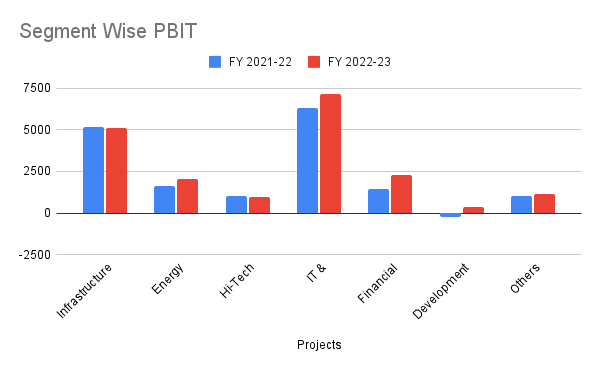
\includegraphics[width=0.8\textwidth]{Segment Wise PBIT.png}
    \caption{Segment Wise PBIT}
  \end{figure}
  

The segment-wise PBIT registered improvement over the
previous year, majorly in Energy Projects, IT\&TS businesses
and Financial Services business. Further, the PBIT of
Development Projects turned positive during the year
primarily due to the value restatement for Nabha Power
Limited (NPL), in line with the improvement in benchmark
valuations due to the visibility of improved profitability and
favourable outcomes of company-specific litigations.

\subsubsection{Other Income}

It mainly consists of profit on the sale of liquid/short-term investments and interest income. Other income at ¢2,929 crore improved by 29.2\% over ¢2,267 crore, reflective of higher investible surpluses and efficient treasury operations.

\subsubsection{Finance Cost}

The interest expense for FY 2022-23 at ¢3,207 crore was marginally higher by 2.6\% over ¢3,126 crore for the previous year. The reduction in average borrowing at a group level was partly offset by an increase in interest rates during the year. Further, refinancing of Hyderabad Metro term loans with market borrowings also contributed to the containment of the interest cost for the year.

\subsubsection{Tax Expense}

The Income Tax charge for FY 2022-23 was higher at ¢4,484 crore by 6.7\% compared to ¢4,204 crore in the previous year on increased profits.

\subsubsection{Exceptional Items}

Exceptional items during the year mainly comprise divestment of the Mutual Fund business of the Financial Services, partially offset by a one-time charge on remeasurement of the wholesale loan assets of the Financial Services segment at fair value. The previous year mainly included divestment gain on the sale of L\&T Uttaranchal Hydropower Limited, partly offset by tax liabilities on the transfer of L\&T-Nxt to the erstwhile Mindtree Limited.

\subsubsection{Consolidated Profit After Tax and EPS}

Consolidated Profit After Tax (PAT) at ¢10,471 crore for FY 2022-23 increased by 20.8\% over the previous year at ¢8,669 crore. The increase is mainly on account of growth in revenues and other income. Consolidated Basic Earnings per Share (EPS) for FY 2022-23 at ¢74.51 improved over the previous year at ¢61.71.

\subsubsection{Return on Consolidated Net Worth}

The Consolidated Net Worth, as at March 31, 2023, at ¢89,326 crore, reflects a net increase of ¢6,918 crore, as compared to the position as at March 31, 2022. The Return on Net Worth (RONW) for FY 2022-23 was higher at 12.2\%, compared to 11.0\% in the previous year, mainly on account of higher profits.

\subsubsection{Liquidity and Gearing}

Cash flow from Operations (including change in loans and advances towards financing activities) increased to ¢22,777 crore as compared to ¢19,163 crore in the previous year, supported by healthy execution and smart working capital management. During the year, additional funds were also generated mainly from the divestment of the Mutual Fund business of the Financial Services business, treasury, and dividend income.

Funds were utilized mainly for repayment of borrowings of ¢4,832 crore, capital expenditure of ¢3,793 crore, and payment of dividend of ¢3,091 crore. Further, funds were applied for the purchase of current investments of ¢8,955 crore and net interest payment of ¢3,047 crore during FY 2022-23.

Consequently, there was a net increase of ¢2,893 crore in the cash balances as at March 31, 2023, compared to the beginning of the financial year.

The total Group borrowings as at March 31, 2023, was lower at ¢118,513 crore, compared to ¢123,468 crore as at March 31, 2022. The major decrease is in borrowings of the Parent entity, Financial Services, and Nabha Power. At a Group level, the gross debt-equity ratio decreased to 1.14:1 as at March 31, 2023, from 1.29:1 as at March 31, 2022. The net debt-equity ratio improved to 0.62:1 as at March 31, 2023, from 0.81:1 as at March 31, 2022.

% \usepackage{tabularray}
\begin{longtblr}[
    caption = {Financial Ratios Comparison},
  ]{
    width = \linewidth,
    colspec = {Q[71]Q[583]Q[90]Q[90]Q[100]},
    column{odd} = {c},
    column{4} = {c},
    hlines,
    vlines,
  }
  \textbf{Sr. No.} & \textbf{Particulars}                                                              & \textbf{FY 21-22} & \textbf{FY 22-23} & \textbf{\% Growth} \\
  (i)              & Gross Debt Equity Ratio                                                           & 1.29              & 1.14              & 11.6\%             \\
  (ii)             & PBDIT as \% of net revenue                                                        & 11.6\%            & 11.3\%            & -2.7\%             \\
  (iii)            & Net Working Capital as \% of Sales (Excluding Financial Services and Corporate)   & 19.7\%            & 16.1\%            & 18.2\%             \\
  (iv)             & Interest Coverage Ratio (excluding Financial Services and Finance Lease Activity) & 5.14              & 5.45              & 6.2\%              
  \end{longtblr}


  \subsection{Strategic Objectives}

\subsubsection{SO-I: Value-accretive growth of current businesses}

\textbf{Performance Measures:}
\begin{itemize}
    \item Revenue growth
    \item Composition of Services in total revenues
\end{itemize}

In FY 2022-23, with a return to normalcy of business activities, the Group achieved revenues of ¢183,341 crore (17\% year-on-year). The Services businesses continued to show strong growth (20\% year-on-year) with a stable percentage share in revenues at 30\% in FY 2022-23.

\subsubsection{SO-II: Scaling-up digital and e-commerce businesses}

\textbf{Performance Measures:}
\begin{itemize}
    \item Growth of digital and e-commerce businesses
\end{itemize}

L\&T Data Center and Cloud Services business has been launched in FY 2022-23 with the commencement of construction of Data Centers in Panvel and Kancheepuram. L\&T-SuFin and L\&T EduTech have been scaled-up further, post their formal launch in FY 2021-22.

\subsubsection{SO-III: Developing business offerings to ride the Energy Transition wave}

\textbf{Performance Measures:}
\begin{itemize}
    \item Size of Green Business
    \item New business or business offering developed
\end{itemize}

The Green Business of L\&T grew to ¢413 billion, which is 37\% of standalone revenues in FY 2022-23 (as compared to 34.7\% in FY 2021-22). The Group also made significant progress in the Green Energy business with the signing of MoUs/agreements (with partners, for the development of Green Hydrogen projects) and setting up a pilot plant for Green Hydrogen production at its Hazira facility.

\subsubsection{SO-IV: Divestment of non-core businesses}

\textbf{Performance Measures:}
\begin{itemize}
    \item Divestment of businesses
\end{itemize}

In FY 2022-23, the Group entered into a Share Purchase Agreement to divest its entire stake in L\&T IDPL (a joint venture having investments in road projects and power transmission assets). The Group continues to actively pursue divestments from other non-core assets and is also exploring various alternatives to derisk the current exposure in Hyderabad Metro.

\subsubsection{SO-V: Enabling business sustainability through a high focus on ESG and Shareholder Value Creation}

\textbf{Performance Measures:}
\begin{itemize}
    \item Metrics linked to ESG performance based on materiality, e.g.,
    \begin{itemize}
        \item Carbon footprint - 29,116 ton CO2 Emissions avoided
        
        \item Resource consumption - 24\%
        Non-Virgin/Recycled and
        eco-friendly materials used
        \item LTIFR (Lost Time Injury Frequency Rate) - 0.06
        LTIFR
        \item Training hours - 6.9 Mn
        Safety training
        man hours
    \end{itemize}
\end{itemize}

\subsection{Sustainability Governance}

The Company conducts materiality assessment (refer to
Materiality Assessment section) to identify and prioritise the
key material topics pertaining to ESG, based on the relative
importance of these topics to the stakeholders and in the
context of L\&T’s business imperatives. The assessment identified
15 important material topics, on the six capitals.
To report sustainability highlights at an overall level, at least
one KPI has been selected for each material topic based on
the importance attached by investors, rating agencies and
regulators and these are given below.

\subsubsection{Environment}

\begin{table}[ht]
    \centering
    \caption{Environment Sustainability Highlights (in various units per ¢ Billion)}
    \begin{tabular}{|l|c|}
    \hline
    \textbf{Sustainability Category} & \textbf{Value} \\
    \hline
    Energy Consumption Intensity & 9,882 GJ/ ¢ Bn \\
    Sourcing from Renewables &  9.6\%\\
    Emissions (GHG Emission Intensity) & 889 tCO2 e/ ¢ Bn \\
    Carbon Sequestration Potential (from Tree Plantation) & 141,300 tCO2 e \\
    Water Consumption Intensity & 10,155 kL/ ¢ Bn \\
    Wastewater Recycling Efficiency & 68\% \\
    Material Management (Recycled and Eco-friendly Material Used) & 24\% \\
    Green Business (Revenue from Green Business) & 37\% \\
    \hline
    \end{tabular}
    \end{table}
    
    % \usepackage{tabularray}

\subsubsection{Social}
\begin{longtblr}[
    caption = {Social Sustainability Highlights},
  ]{
    width = \linewidth,
    colspec = {Q[846]Q[96]},
    column{2} = {c},
    vlines,
    hline{1-2,12} = {-}{},
  }
  \textbf{Sustainability Category}                                                  & \textbf{Value} \\
  Health and Safety (Safety Training Man Hours)                                     & 6.9 Mn         \\
  Health and Safety (LTIFR1)                                                        & 0.06           \\
  Human Rights (Own Locations Assessed and Complied with Human Rights Requirements) & 100\%          \\
  Workforce Skilling and Talent Management (Employees)                              & 28,000+        \\
  Workforce Skilling and Talent Management (Workers Trained on Skill Upgradation)   & 45,000+        \\
  Workforce Skilling and Talent Management (Attrition Rate)                         & 13.9\%         \\
  Diversity and Inclusion (Diversity)                                               & 7.1\%          \\
  Diversity and Inclusion (Women in Senior Management)                              & 89             \\
  Social Impact (CSR Beneficiaries)                                                 & 1.5 Mn         \\
  Social Impact (MSME Suppliers)                                                    & 10,736         
  \end{longtblr}

\subsubsection{Governance}
    % \usepackage{color}
% \usepackage{tabularray}
\begin{longtblr}[
    caption = {Governance and Ethics Sustainability Highlights},
  ]{
    width = \linewidth,
    colspec = {Q[867]Q[75]},
    cell{1}{2} = {c},
    cell{2}{2} = {c},
    cell{3}{2} = {c},
    cell{4}{2} = {c},
    cell{5}{2} = {c},
    cell{6}{2} = {c},
    cell{7}{2} = {c},
    cell{8}{2} = {c},
    vlines,
    hline{1-2,8-10} = {-}{},
  }
  \textbf{Sustainability Category}                                                             & \textbf{Value} \\
  Governance  Ethics (New Joinees Trained on CoC)                                              & 100\%          \\
  Customer Centricity (Customer Satisfaction Score out of 10)                                  & 9.2            \\
  Data Privacy  Cyber Security                                                                 & 0              \\
  Sustainable Supply Chain (Sustainable Sourcing of Input Material from Neighboring Districts) & 40\%           \\
  Sustainable Supply Chain (Sustainable Value of Input Material Sourced from Suppliers)        & 7\%            \\
  Brand Management (Ranked among 'World's Top 200 Environmental Firms' by ENR for 2022)        & 3rd            \\
  Brand Management (Certified as Great Place To Work®)                                         &                \\
  New Policies (Anti Bribery and Anti Corruption, Equal Opportunity, Public Policy Advocacy)   &                
  \end{longtblr}

\subsection{Long-term commitment }

\subsubsection{NATURAL CAPITAL}
\begin{itemize}
  \item Water consumption: 11 Mn kL
  \item Energy from Non-Renewable sources: 10.61 Mn GJ 
  \item Energy from Renewable sources: 0.13 Mn GJ
  \item Spend on Environment: \$288.4 Mn 
  \item Material consumed \(Mn tonnes\):
    \begin{itemize}
      \item Cement: 4.61 
      \item Sand: 6.95 
      \item Ferrous: 3.06
    \end{itemize}
\end{itemize}

\subsubsection{MANUFACTURED CAPITAL}
\begin{itemize}
  \item Active Project Sites: 729 
  \item Manufacturing plants: 18
\end{itemize}

\subsubsection{SOCIAL AND RELATIONSHIP CAPITAL}
\begin{itemize}
  \item CSR spend: ¢ 1.4 Bn 
  \item CSR partners: 64
  \item MSME suppliers: 10,736
  \item Memberships of Industry Chambers: 75
\end{itemize}

\subsubsection{HUMAN CAPITAL}
\begin{itemize}
  \item Employees: 55,202
  \item Engineers: 41,000 
  \item Workmen: 277,857 
  \item Employees covered under Leadership Development Programmes: 1,672
\end{itemize}

\subsubsection{FINANCIAL CAPITAL}
\begin{itemize}
  \item Order Book: \$3,305.5 Bn
  \item Net Current Assets: \$324.9 Bn 
  \item Net Fixed Assets: \$117.1 Bn
\end{itemize}

\subsubsection{INTELLECTUAL CAPITAL}
\begin{itemize}
  \item R\&D spend (cumulative last 3 years): \$3,448 Mn 
  \item Patents filed: 8
  \item R\&D Engineers and Scientists: 380
  \item Active collaborations and partnerships: 20
\end{itemize}



\section{Technology Venturing at IBM}

IBM is a global leader in technology innovation, and its involvement in technology venturing and startups is a key component of its strategy to maintain its competitive edge. This report discusses IBM's investments, acquisitions, and partnerships with technology startups, along with the impact on the company's growth and innovation.

\subsection{Investments}

IBM Ventures invests in startups across various technology sectors, including artificial intelligence, cloud computing, cybersecurity, blockchain, and quantum computing. IBM Ventures typically participates in Series A and B rounds, with investment amounts ranging from $1 million to $10 million.

In recent years, IBM Ventures has invested in several high-profile startups, including:

\begin{itemize}
    \item \textbf{Scale AI:} A startup specializing in machine learning models for large enterprises.
    \item \textbf{Cloudinary:} A cloud-based image and video management services provider.
    \item \textbf{Arkose Labs:} A startup developing fraud prevention solutions for online businesses.
    \item \textbf{Chainalysis:} A provider of blockchain intelligence and analytics software.
    \item \textbf{Rigetti Computing:} A startup focusing on quantum computers.
\end{itemize}

\subsection{Acquisitions}

IBM also acquires technology startups to gain access to new technologies, talent, and markets. IBM's acquisition strategy aims to complement its existing product portfolio and accelerate its growth.

In recent years, IBM has acquired several high-profile startups, including:

\begin{itemize}
    \item \textbf{Red Hat:} A leading open-source software provider.
    \item \textbf{Watson Analytics:} A startup with a cloud-based data analytics platform.
    \item \textbf{Cleversafe:} A startup offering a cloud-based object storage platform.
    \item \textbf{SoftLayer:} A startup providing cloud computing services.
    \item \textbf{Trusteer:} A startup specializing in security software for online banking and shopping websites.
\end{itemize}

\subsection{Partnerships}

IBM also partners with technology startups to accelerate the development and commercialization of new products and services. IBM's partnership strategy focuses on collaborating with startups that have complementary technologies and share IBM's vision for the future of technology.

In recent years, IBM has partnered with several high-profile startups, including:

\begin{itemize}
    \item \textbf{Google Cloud:} IBM and Google Cloud offer joint solutions and services to enterprise customers.
    \item \textbf{Microsoft Azure:} IBM and Microsoft Azure provide joint solutions and services to enterprise customers.
    \item \textbf{Amazon Web Services:} IBM and Amazon Web Services collaborate on joint solutions and services for enterprise customers.
    \item \textbf{Salesforce:} IBM and Salesforce deliver joint solutions and services to enterprise customers.
    \item \textbf{SAP:} IBM and SAP partner to offer joint solutions and services to enterprise customers.
\end{itemize}

\subsection{Impact on IBM's Growth and Innovation}

IBM's involvement in technology venturing and startups has had a significant impact on the company's growth and innovation. IBM's investments in startups have helped the company stay ahead in emerging technologies, such as artificial intelligence, cloud computing, and cybersecurity. IBM's acquisitions of startups have allowed the company to expand its product portfolio and enter new markets. Furthermore, IBM's partnerships with startups have accelerated the development and commercialization of new products and services.

Specific examples of the impact include:

\begin{itemize}
    \item IBM's acquisition of Red Hat helped the company become a leader in the open-source software market.
    \item IBM's investment in Scale AI accelerated the development of machine learning technologies.
    \item IBM's partnership with Google Cloud expanded its range of cloud computing services for customers.
    \item IBM's acquisition of SoftLayer facilitated the expansion of its cloud computing business.
    \item IBM's partnership with Microsoft Azure broadened the range of cloud computing services for customers.
\end{itemize}


\section{Sustainability of Technology/Firm: IBM's Initiatives and ESG Considerations}

IBM is committed to sustainability and has several initiatives in place to reduce its environmental impact, improve its social performance, and uphold its ethical values. IBM's sustainability initiatives are aligned with the United Nations Sustainable Development Goals (SDGs).

\subsubsection{Environmental Initiatives}

IBM's environmental sustainability initiatives include:

\begin{itemize}
    \item \textbf{Net-Zero Greenhouse Gas Emissions by 2030:} IBM has set a goal to achieve net-zero greenhouse gas emissions by 2030.
    \item \textbf{100\% Renewable Energy:} IBM is committed to using 100\% renewable energy.
    \item \textbf{Water Consumption Reduction:} IBM aims to reduce its water consumption.
    \item \textbf{Energy-Efficient Technologies:} IBM has developed energy-efficient technologies, such as its Green Horizons power management software.
\end{itemize}

\subsubsection{Social Initiatives}

IBM's social sustainability initiatives include:

\begin{itemize}
    \item \textbf{Diversity and Inclusion:} IBM is committed to promoting diversity and inclusion in the workplace.
    \item \textbf{Education and Skills Development:} IBM supports education and skills development programs.
    \item \textbf{Corporate Social Responsibility:} IBM has various corporate social responsibility programs focusing on helping disadvantaged communities.
\end{itemize}

\subsubsection{Governance Initiatives}

IBM's governance initiatives include:

\begin{itemize}
    \item \textbf{Code of Conduct:} IBM has a code of conduct that all employees must follow.
    \item \textbf{Board of Directors:} IBM has a board of directors that oversees the company's governance practices.
\end{itemize}

\subsection{Environmental, Social, and Governance (ESG) Considerations in Technology Management}

ESG considerations are becoming increasingly important in technology management, with pressure from investors, customers, and employees to improve sustainability performance.

\subsubsection{ESG Considerations}

Key ESG considerations in technology management include:

\begin{itemize}
    \item \textbf{Environment:} Technology companies must reduce their environmental impact by using renewable energy, reducing waste production, and developing energy-efficient technologies.
    \item \textbf{Social:} Promoting diversity and inclusion in the workplace, supporting education and skills development programs, and addressing potential negative social impacts are crucial for technology companies.
    \item \textbf{Governance:} Technology companies require a strong governance framework to ensure ethical and responsible operations.
\end{itemize}

\subsection{The Role of Sustainability in the Long-Term Success of IBM}

Sustainability is essential for IBM's long-term success. It contributes to talent attraction, customer retention, and cost reduction.

\subsubsection{Role of Sustainability}

Sustainability contributes to IBM's long-term success in the following ways:

\begin{itemize}
    \item \textbf{Talent Attraction and Retention:} Sustainability initiatives help IBM attract and retain top talent, as employees are increasingly interested in working for a sustainable company.
    \item \textbf{Customer Attraction and Retention:} Customers prefer doing business with companies committed to sustainability, and IBM's initiatives help attract and retain customers.
    \item \textbf{Cost Reduction:} Sustainability initiatives, such as energy efficiency, help IBM reduce costs, including energy expenses.
\end{itemize}



\chapter{Discussions and conclusion}
In this chapter, the work is concluded and future plan is presented and the limitation of the work and possible future extensions are
described respectively.

\section{Final Conclusion} In this study, we use deep learning techniques to directly optimise the Sharpe ratio of a portfolio. By updating model parameters via gradient ascent, this pipeline avoids the limitations of conventional forecasting and enables us to better manage portfolio weights. BSE Sensex has been utilised as the benchmark portfolio in this study.
We contrast our approach with other well-known techniques, such as risk parity optimisation, maximum diversification, classical mean-variance optimisation reallocation techniques.
Our testing period, which runs from January 2000 to July 2022, encompasses the current COVID-19 situation.
The outcomes demonstrate that our model offers the greatest performance, and a thorough analysis of our model's performance in the actual scenario demonstrates the logic and viability of our approach.
\section{Contribution}
This study contributes to the field since there is no publication in the literary works that extensively and collectively covers the following topics: practical limitations, probabilistic and analytical approaches, different forms of performance evaluation, evaluation of strategy using back testing , and use of programming language and Deep Learning.\\\\
\section{Limitations}
There are two major limitations in this study that could be addressed in future research. \begin{itemize}
    \item Current Study Parameters can only include one Benchmark
    \item The study focused on only stock portfolios while there are many different types of assets whose value is appreciated over time.
    \item The stock data availability limits this study at the start of the benchmark period as stocks get listed at a different point in time
    
\end{itemize} 

\section{Future scope}
The next phase of this endeavour will include:
\begin{itemize}

\item Our goal is to examine portfolio performance using various objective functions. We may optimise the Sortino ratio or any other metric of the efficiency of the portfolio because to the flexible framework of our methodology.

\item We will Concentrate to build a portfolio utilising ETFs and market indexes rather than using individual assets. This significantly lowers the range of available assets, and these indexes have shown strong correlations.

\item Instead of just one, Our Technique can also include more market indices and sector-specific indices for Benchmarking Process
\end{itemize}
%\textcolor{white}{"}
%%%%%%%%%%%%%%%%%%%%%%%%%%%%%%%%%%%%%%%%%%%%%%%%%%%%%%%%%%%%%%%%%%%%%%%%%%%%%%
\setcitestyle{round}
% \addcontentsline{toc}{chapter}{REFERENCES}
\bibliographystyle{kluwer}
\bibliography{ref}
\end{document}
